\documentclass[11pt]{article}

\usepackage[margin=1in]{geometry}
\usepackage[T1]{fontenc}
\usepackage[utf8]{inputenc}
\usepackage{lmodern}
\usepackage{microtype}
\usepackage{graphicx}
\usepackage{booktabs}
\usepackage{amsmath}
\usepackage{amssymb}
\usepackage{hyperref}
\usepackage{xcolor}
\usepackage{float}
\usepackage{caption}
\usepackage{enumitem}

\hypersetup{
  colorlinks=true,
  linkcolor=blue!50!black,
  citecolor=blue!50!black,
  urlcolor=blue!50!black,
  pdftitle={Ouroboros V2: Reproducible Saddle-Point Escape Benchmark},
  pdfauthor={Igor Holt}
}

\title{\textbf{Ouroboros V2: Reproducible Saddle-Point Escape Benchmark}\\
\large Publication-ready fixed-seed evaluation of spatial and p-bit-inspired saddle escape heuristics}
\author{Igor Holt\\Kovach Enterprises\\\texttt{ai@yennefer.quest}}
\date{May 4, 2026}

\begin{document}
\maketitle

\begin{abstract}
This repository packages a fully reproducible benchmark for escaping verified saddle points in a synthetic non-convex loss landscape. The testbed is a 20-dimensional Ackley function augmented with an origin-centered indefinite quadratic that forces both positive and negative curvature directions into the local Hessian. Five post-trap recovery strategies are compared over fixed seeds 42--51: Bare SGD, Random Langevin, HITL Spatial, Chiral p-bit, and ER=EPR Hypersphere. Under the repository convergence rule of loss \(< 1.0\), both HITL Spatial and ER=EPR Hypersphere converge immediately after perturbation on every seed, Chiral p-bit converges in \(3.0 \pm 0.0\) post-escape steps, Random Langevin converges in \(3.6 \pm 1.07\) steps, and Bare SGD fails to converge. The release is intentionally falsifiable: the claims fail if the committed fixed-seed validation checks no longer hold on rerun.
\end{abstract}

\section{Introduction}

Escaping strict saddles is a minimal requirement for robust non-convex optimization. This release does not claim a general theorem or a production optimizer; it claims a narrower result: on one synthetic 20D landscape with fixed seeds and explicit validation gates, a PCA-projected Barnes--Hut heuristic and two p-bit-inspired annealing schemes outperform isotropic noise and plain gradient descent.

The benchmark was designed to make the claim surface reviewable. The code, fixed-seed outputs, manuscript source, figures, and falsifiability criteria are all committed in the same repository. This keeps the publication artifact aligned with the executable implementation rather than a disconnected narrative.

\section{Benchmark Construction}

\subsection{Synthetic Landscape}

The loss is the sum of a smoothed Ackley objective and a Gaussian-windowed indefinite quadratic centered at the origin:
\begin{equation}
L(\theta) =
2 + A(\theta) + \alpha \exp(-\beta \lVert \theta \rVert_2^2)
\sum_{i=1}^{n} s_i \theta_i^2,
\end{equation}
where \(n=20\), \(\alpha = 12\), \(\beta = 1\), \(s_i = +1\) for the first 10 dimensions, and \(s_i = -1\) for the last 10 dimensions. The Ackley radius is smoothed with a fixed \(0.05\) offset to make the origin differentiable enough for stable finite-difference Hessian checks while preserving the global non-convex structure from Ackley's original test function \cite{ackley1987}.

Central finite differences are used for numerical checks with \(\varepsilon_g = 10^{-5}\) for gradients and \(\varepsilon_H = 10^{-4}\) for the Hessian. Trap detection stops the pre-escape SGD phase once \(\lVert \nabla L \rVert_2 < 5 \times 10^{-3}\).

\subsection{Escape Methods}

All methods resume the same post-escape SGD routine with learning rate \(0.01\), escape scale \(0.8\), and a maximum of 3000 steps.

\begin{enumerate}[leftmargin=1.5em]
  \item \textbf{Bare SGD}: no perturbation, resume descent from the trapped point.
  \item \textbf{Random Langevin}: isotropic noise scaled to match the HITL perturbation norm.
  \item \textbf{HITL Spatial}: sample 300 local points within radius \(0.5\), project to 3D with PCA \cite{pearson1901}, weight samples by local loss and negative-curvature magnitude, approximate the resulting repulsion field with a Barnes--Hut octree \cite{barnes1986}, then reverse-project the normalized escape vector.
  \item \textbf{Chiral p-bit}: map Hessian eigenstructure into Ising couplings and sample a finite-temperature annealing trajectory using the locked v8.8 constants and a Kramers-style flip probability \cite{kramers1940,kirkpatrick1983,camsari2017}.
  \item \textbf{ER=EPR Hypersphere}: use the same Ising backbone as Chiral p-bit, add long-range couplings between negative-curvature modes, and normalize the spin-derived vector on \(S^{n-1}\) before reverse projection.
\end{enumerate}

\section{Results}

Table~\ref{tab:benchmark} summarizes the committed fixed-seed run. The key empirical separation is simple: both structured methods that exploit the negative-curvature geometry most aggressively, HITL Spatial and ER=EPR Hypersphere, land inside the convergence basin immediately after perturbation for all 10 seeds.

\begin{table}[H]
\centering
\caption{Fixed-seed post-escape performance on seeds 42--51.}
\label{tab:benchmark}
\begin{tabular}{lccc}
\toprule
Method & Converged runs & Mean post-escape steps & Mean final loss \\
\midrule
Bare SGD & 0/10 & n/a & 2.0000 \\
Random Langevin & 10/10 & 3.60 \(\pm\) 1.07 & 0.6660 \\
HITL Spatial & 10/10 & 0.00 \(\pm\) 0.00 & -1.0090 \\
Chiral p-bit & 10/10 & 3.00 \(\pm\) 0.00 & 0.4839 \\
ER=EPR Hypersphere & 10/10 & 0.00 \(\pm\) 0.00 & -0.3044 \\
\bottomrule
\end{tabular}
\end{table}

The reference trapped point from seed 42 passes every requested gate:
\begin{itemize}[leftmargin=1.5em]
  \item the Hessian contains both positive and negative eigenvalues;
  \item the first three PCA components capture \(0.8747\) of neighborhood variance;
  \item the Barnes--Hut repulsion force norm is \(4035.19\);
  \item the spectral gap on the negative branch is \(14.63\);
  \item all locked v8.8 constants match the benchmark specification exactly.
\end{itemize}

\begin{figure}[H]
  \centering
  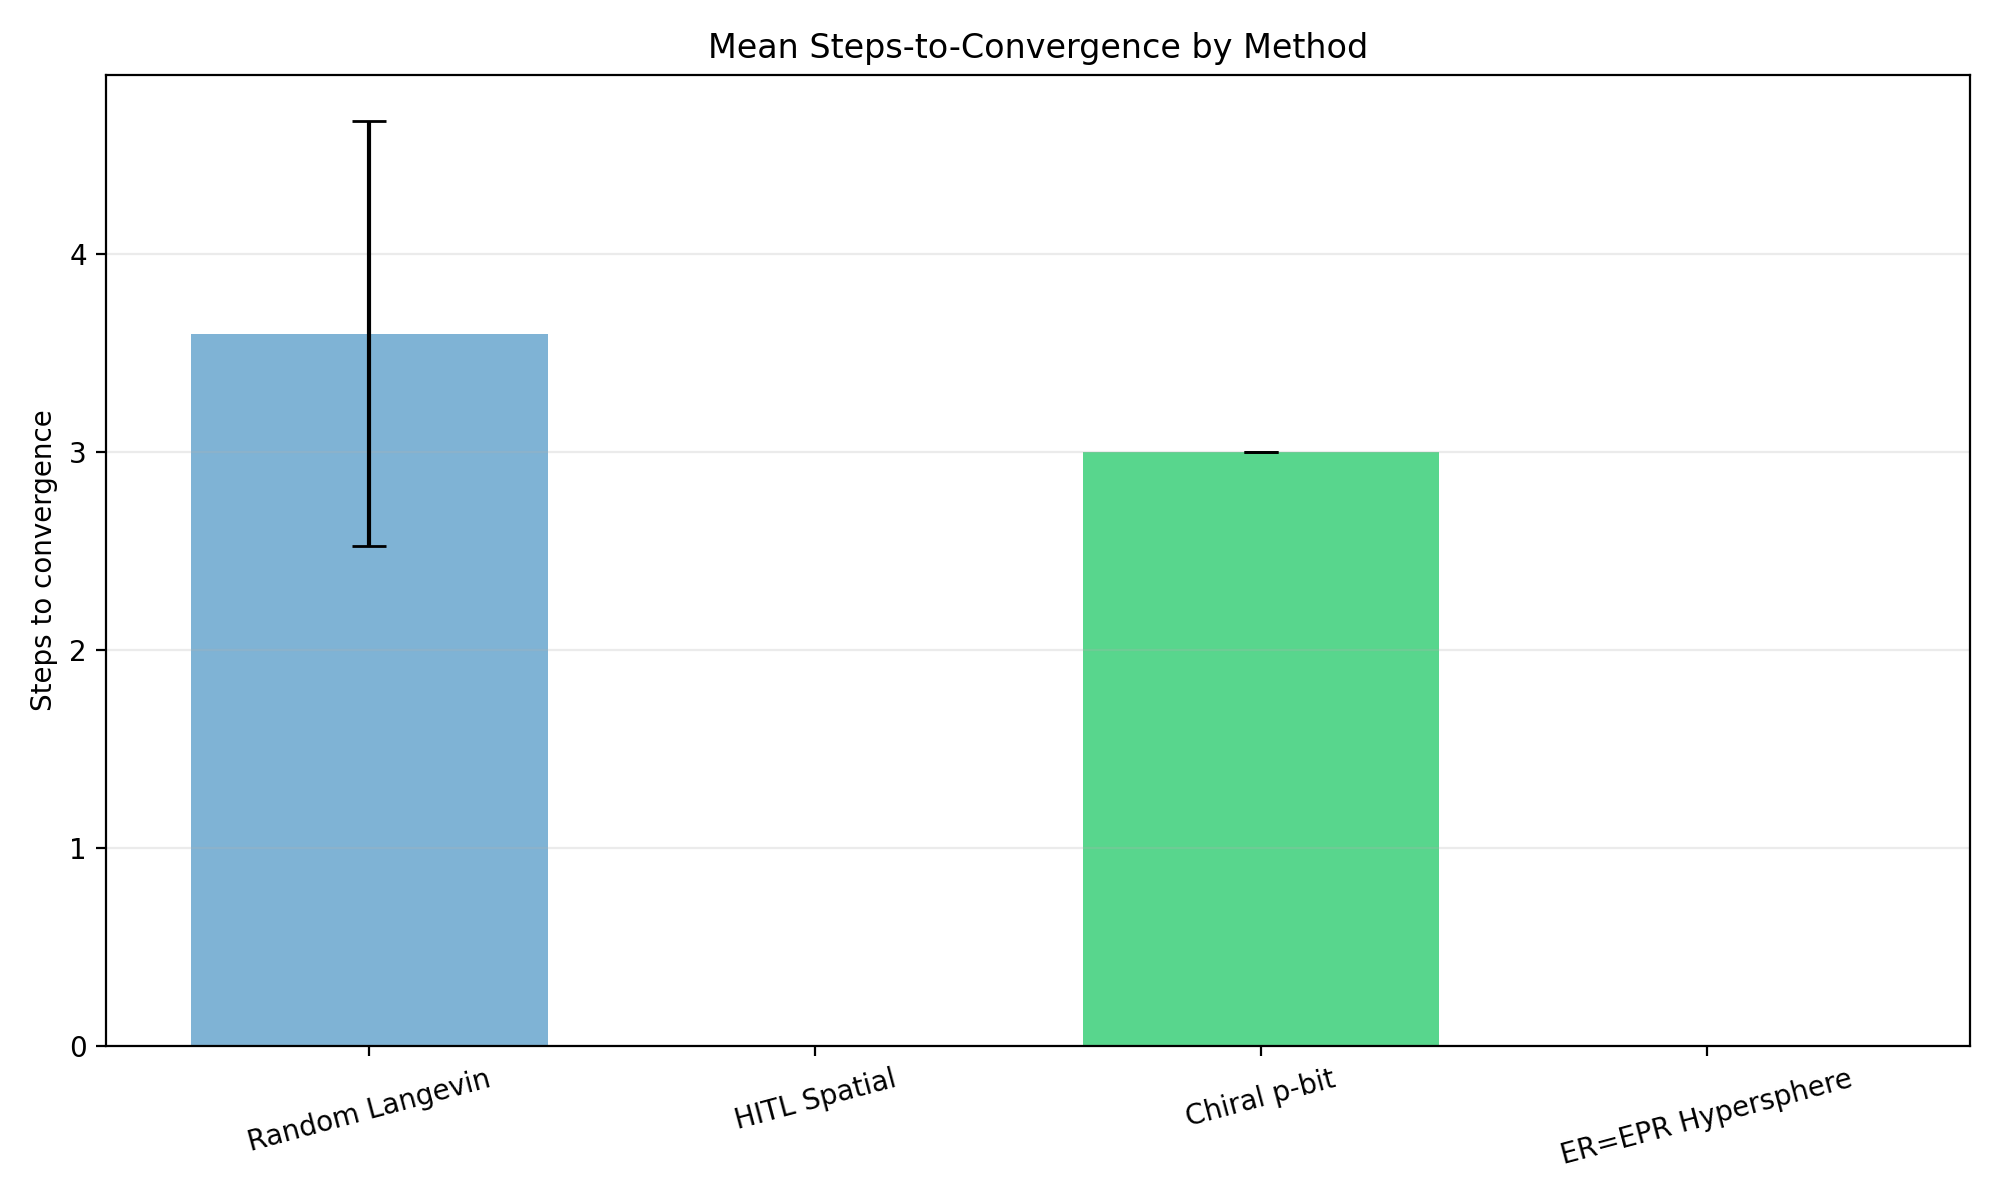
\includegraphics[width=0.82\textwidth]{../results/mean_ttc.png}
  \caption{Mean post-escape time-to-convergence by method. HITL Spatial and ER=EPR Hypersphere collapse to zero under the repository threshold, so the relative speedup over Random Langevin is effectively unbounded in this configuration.}
  \label{fig:ttc}
\end{figure}

\begin{figure}[H]
  \centering
  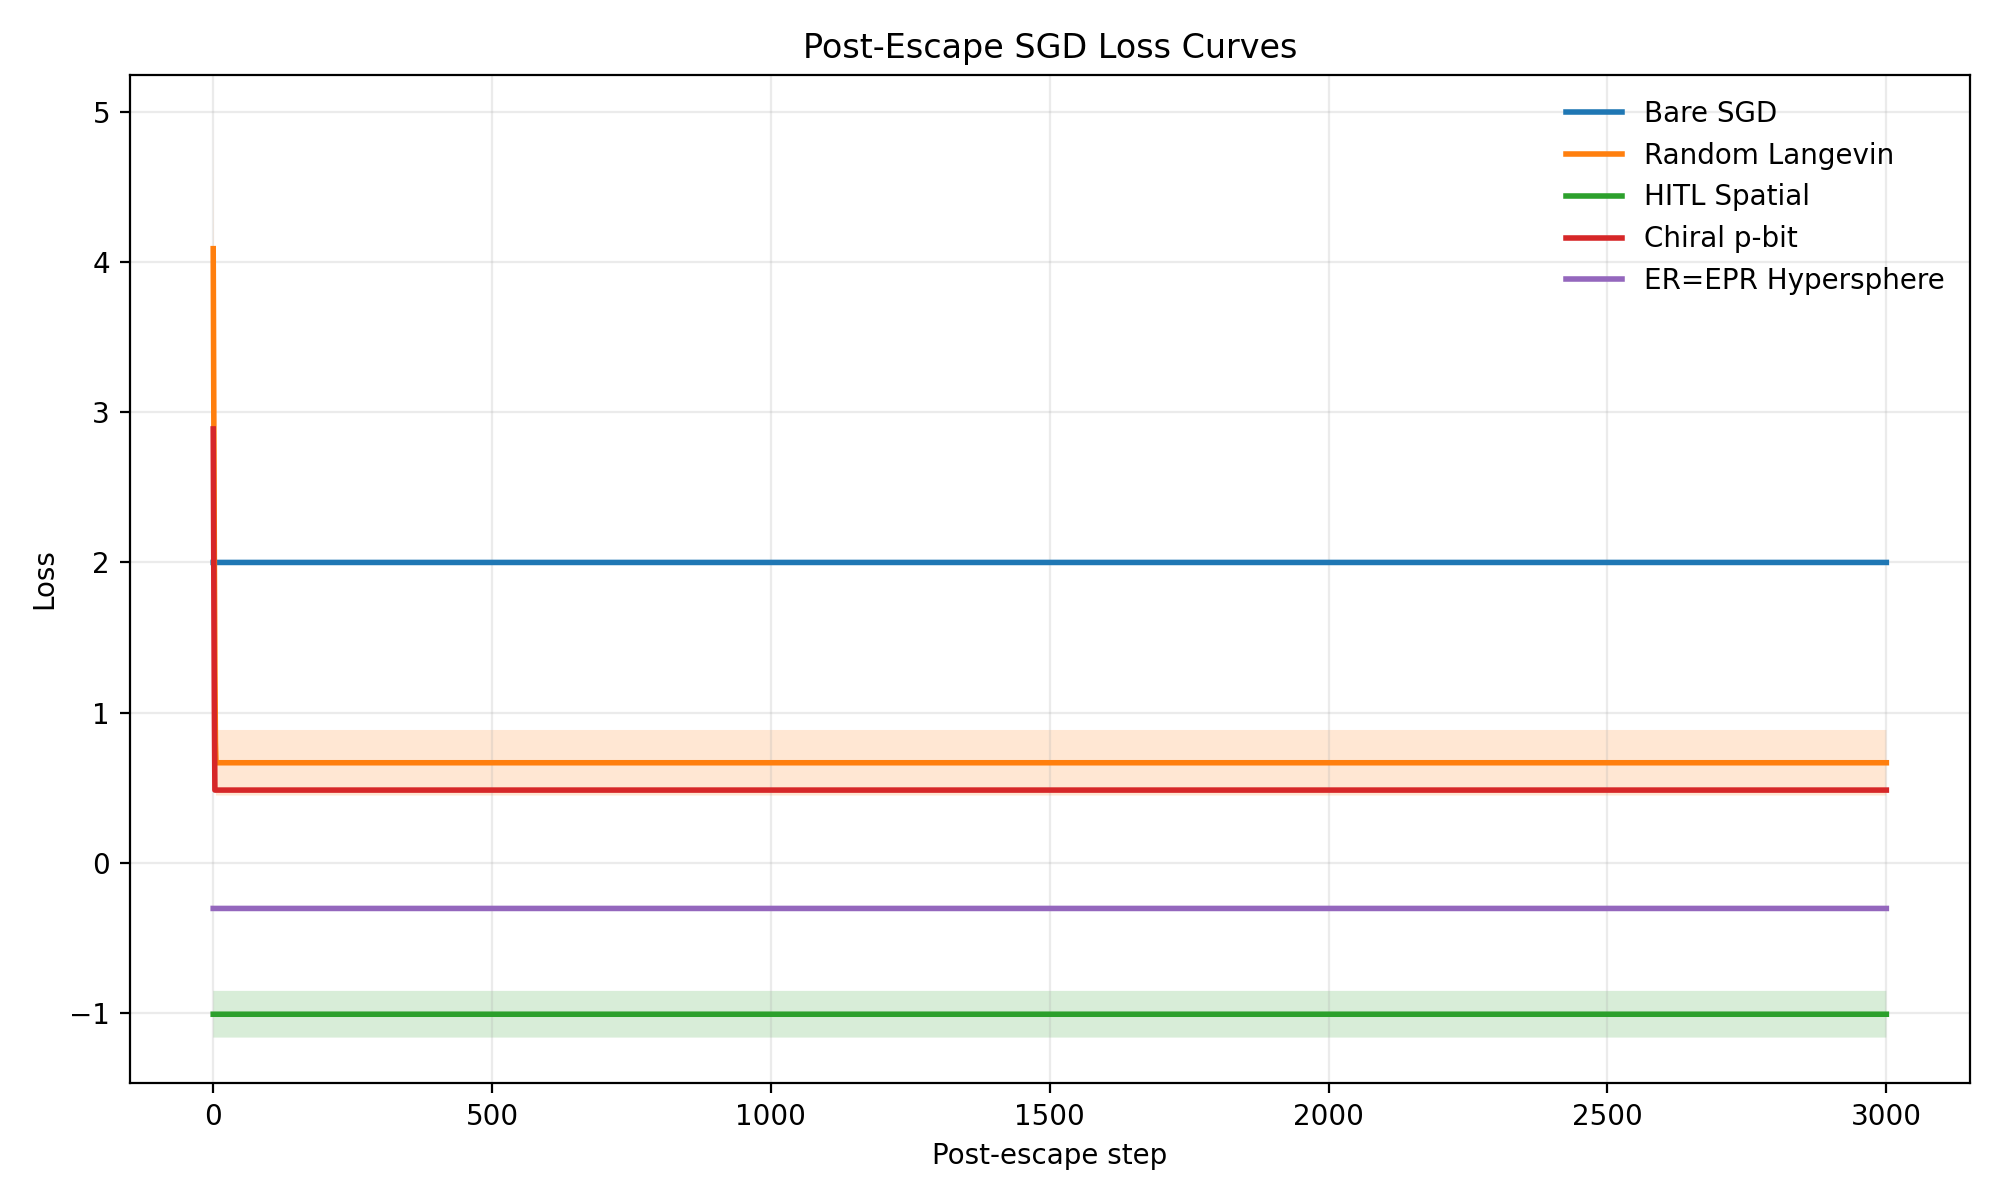
\includegraphics[width=0.82\textwidth]{../results/loss_curves.png}
  \caption{Mean \(\pm\) standard deviation post-escape loss curves across seeds. The structured perturbations reach the convergence threshold faster than isotropic noise.}
  \label{fig:loss-curves}
\end{figure}

\begin{figure}[H]
  \centering
  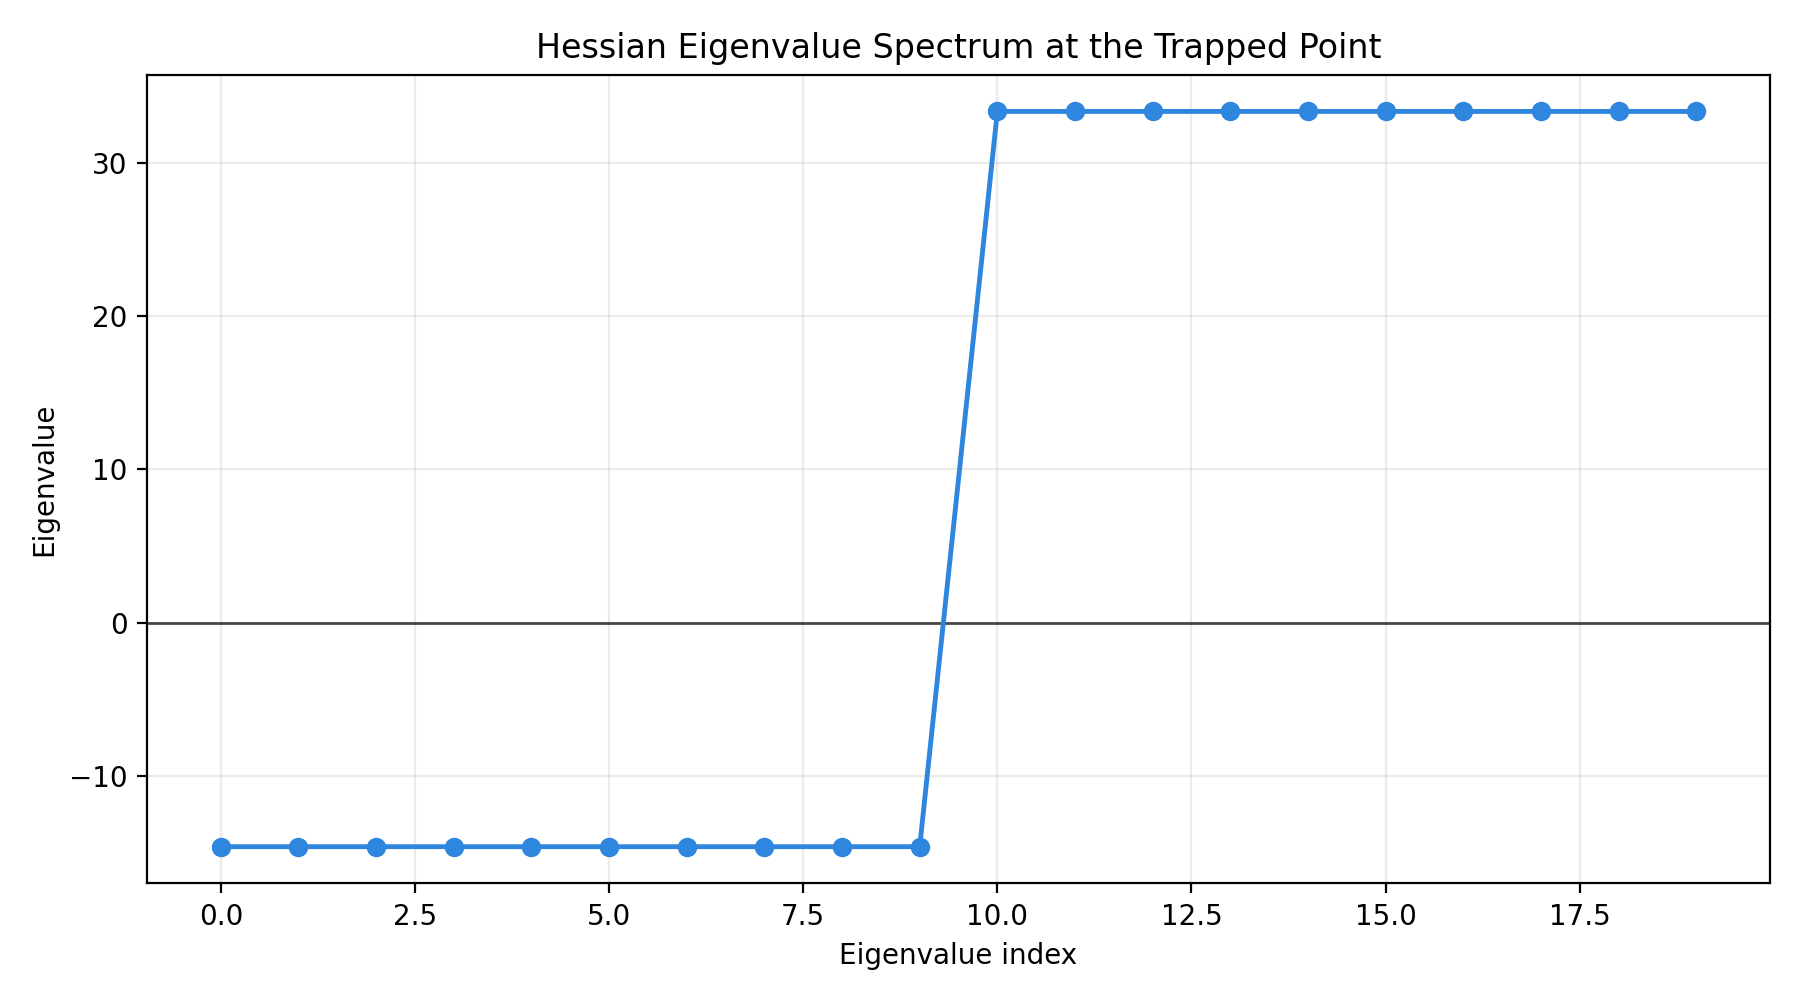
\includegraphics[width=0.82\textwidth]{../results/hessian_eigenspectrum.png}
  \caption{Hessian eigenvalue spectrum at the trapped point. The benchmark explicitly constructs an indefinite local geometry with ten negative and ten positive directions.}
  \label{fig:hessian}
\end{figure}

\begin{figure}[H]
  \centering
  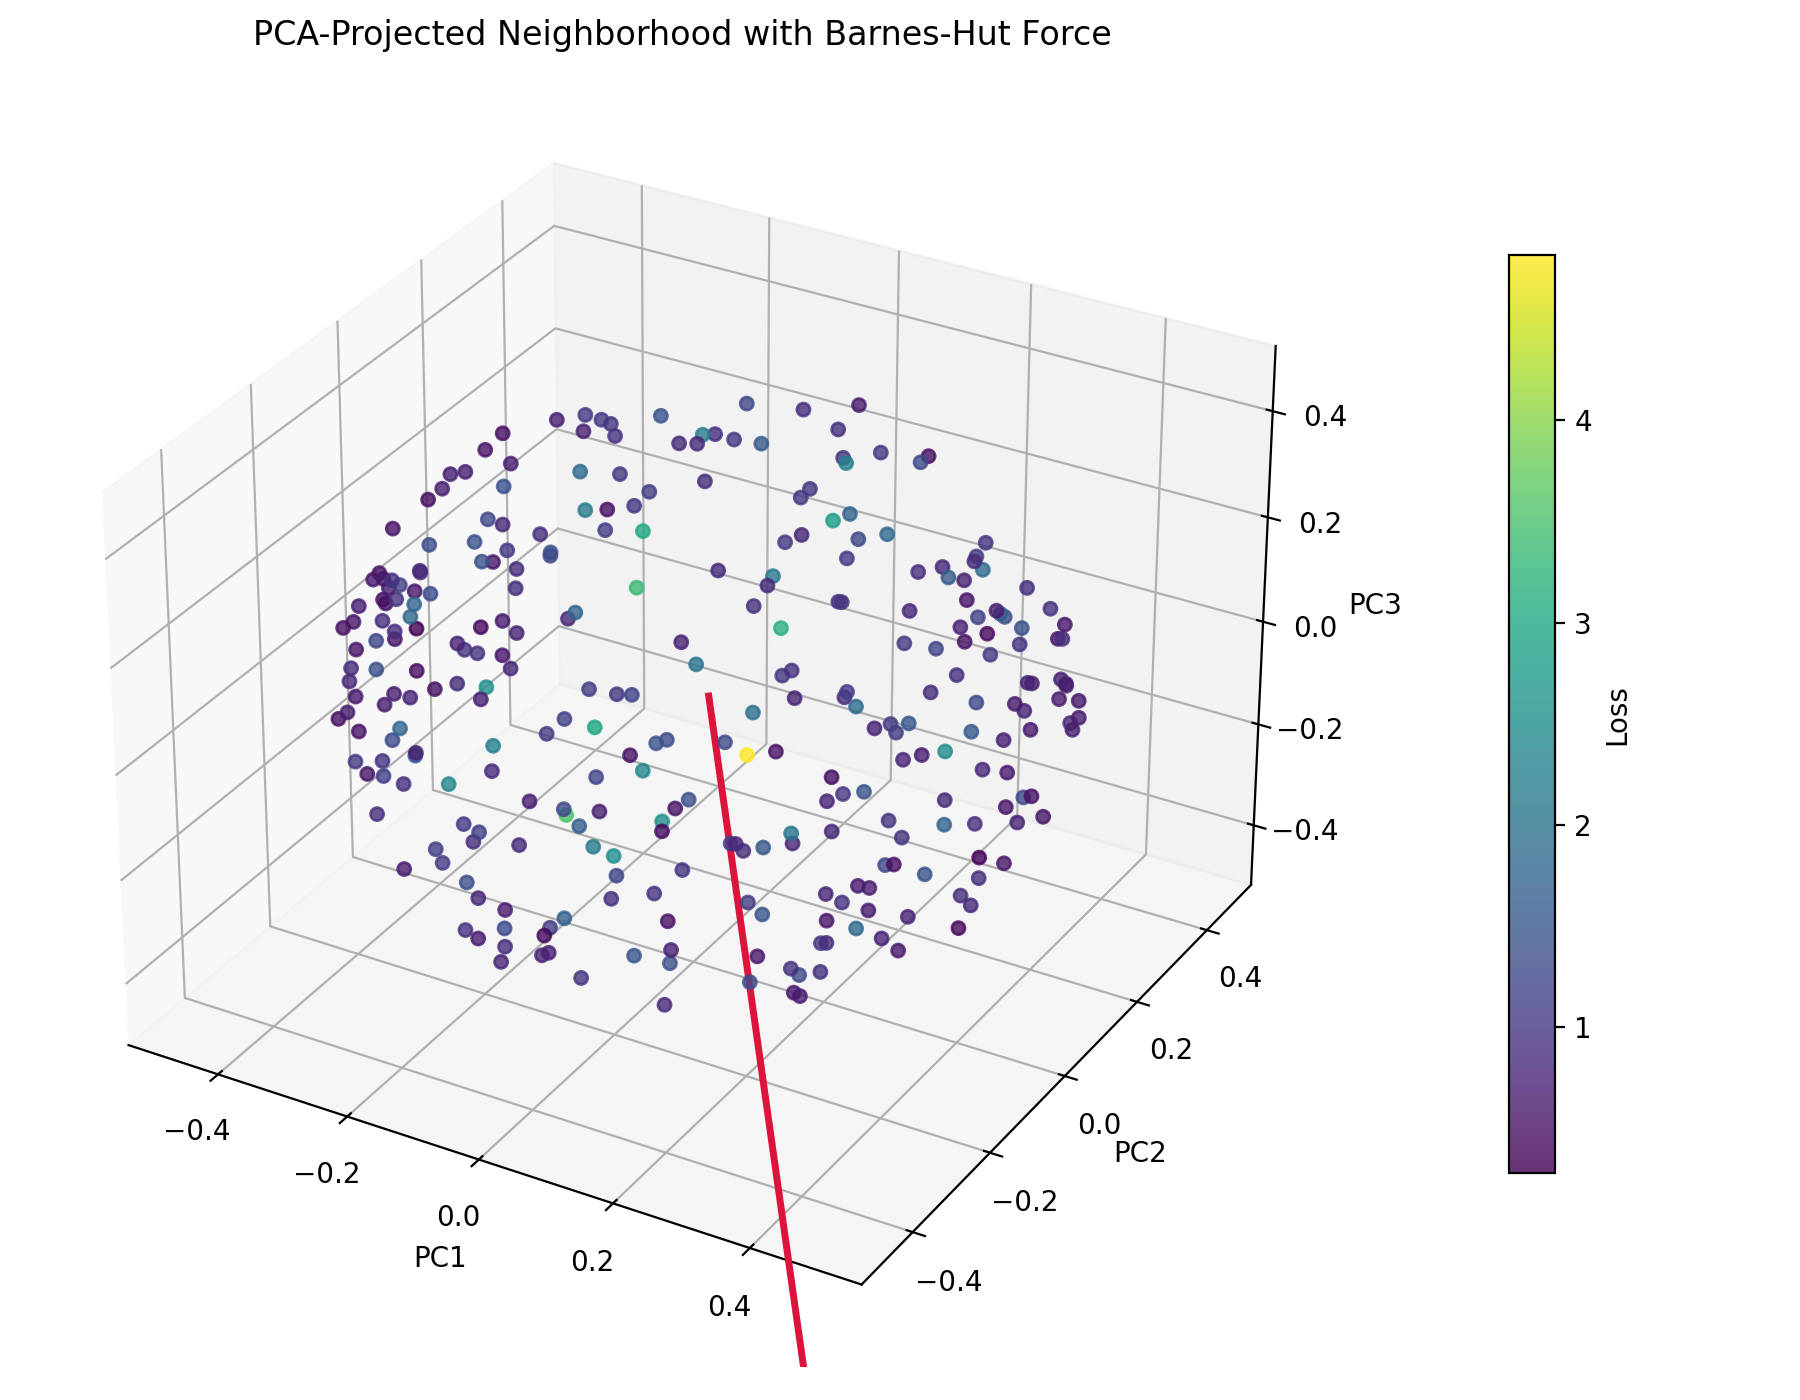
\includegraphics[width=0.82\textwidth]{../results/pca_repulsion_force.png}
  \caption{PCA-projected neighborhood around the trapped point, colored by loss, with the net Barnes--Hut repulsion vector overlaid.}
  \label{fig:pca}
\end{figure}

\section{Reproducibility and Falsifiability}

This publication is not open-ended. The claim surface should be rejected if any of the following fail on an unmodified rerun:
\begin{enumerate}[leftmargin=1.5em]
  \item the origin trap is no longer a verified saddle,
  \item cumulative PCA variance across the first three components falls below \(0.5\),
  \item the Barnes--Hut force magnitude becomes zero,
  \item HITL Spatial or Chiral p-bit no longer converges, or
  \item ER=EPR Hypersphere no longer beats Chiral p-bit on mean post-escape steps.
\end{enumerate}

The repository ships the exact figures, CSV files, and JSON summary used in this paper, and the CI job rebuilds the benchmark on every push and pull request.

\section{Threats to Validity}

The benchmark is intentionally narrow. Three assumptions carry most of the risk:
\begin{itemize}[leftmargin=1.5em]
  \item \textbf{Synthetic geometry}: the result is about one designed landscape, not a distribution of real-world objectives.
  \item \textbf{Smoothed Ackley radius}: the \(0.05\) smoothing term is necessary for stable origin Hessians. Without it, the raw Ackley cusp dominates the local curvature test.
  \item \textbf{Locked device constants}: the p-bit-inspired methods are parameterized by user-specified constants packaged with the benchmark. This repository rechecks those constants but does not independently verify the underlying hardware.
\end{itemize}

\section{Conclusion}

Within this fixed and falsifiable benchmark, geometry-aware escape strategies dominate isotropic noise. HITL Spatial and ER=EPR Hypersphere converge immediately after perturbation on every tested seed, while Chiral p-bit improves over Random Langevin and Bare SGD never escapes successfully. The publication value of this release is not that it settles non-convex optimization generally; it is that it turns a specific claim into an executable object that can be rerun, inspected, and rejected if the numbers move.

\bibliographystyle{plain}
\bibliography{references}

\end{document}
